\section{Inicio de Sesión}

    \subsection{Ingresar al sistema}
        Para poder iniciar sesión en el sistema, debe ingresar la url: \url{https://softwareengineerescom.gitlab.io/APMS/public/login} y podrá ver la siguiente pantalla:

        % Imagen de Iniciar sesión
        \begin{figure}[!hbtp]
            \centering
            \hypertarget{iniciarS}{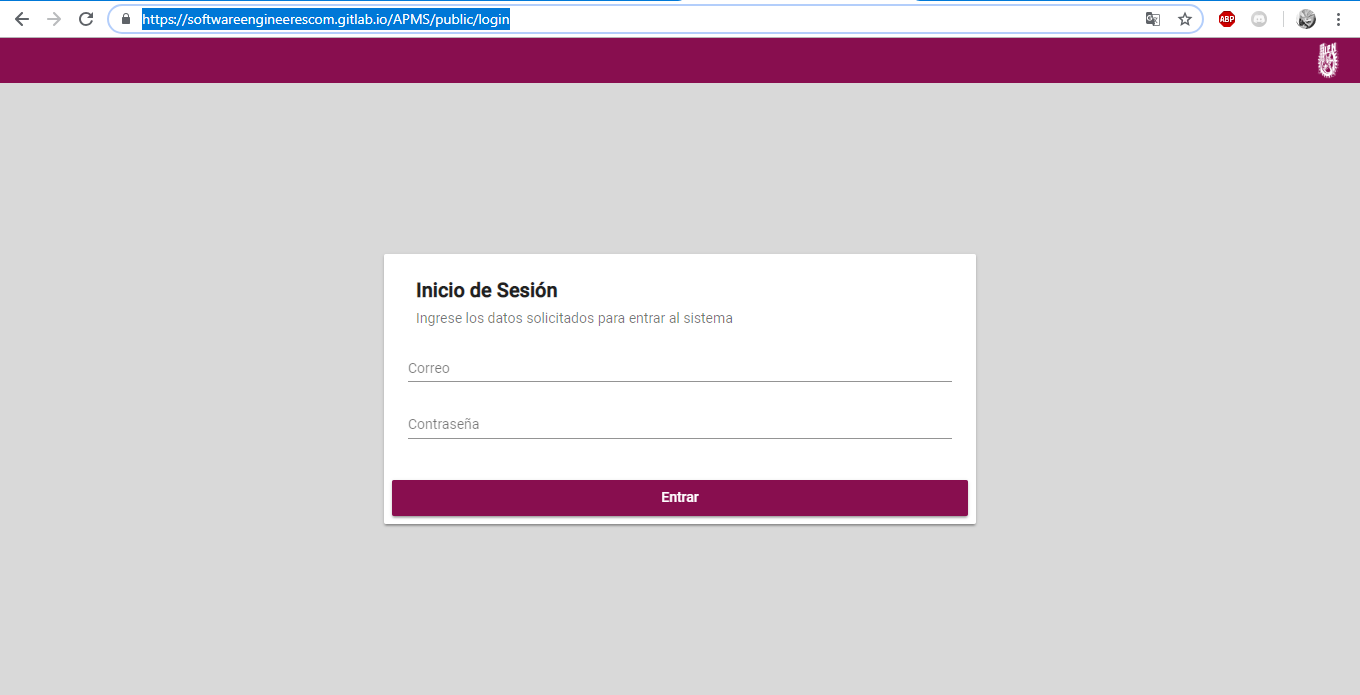
\includegraphics[width=0.7\linewidth]{images/SP5/IniciarSesion}}
            \caption{Pantalla para iniciar sesión}
            %\label{consultarrh}
        \end{figure}
        \clearpage
        Para poder ingresar sesión debe tener su correo electrónico (generalmente institucional) y contraseña que su jefe directo le dio, dichos datos se ingresarán como en el ejemplo que se muestra abajo.

        % Imagen de Iniciar sesión con llenado
        \begin{figure}[!hbtp]
            \centering
            \hypertarget{iniciarL}{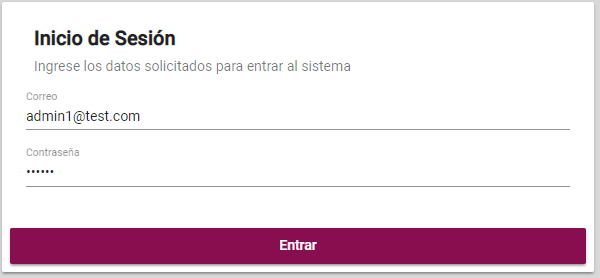
\includegraphics[width=0.5\linewidth]{images/SP5/ejemploIniciar}}
            \caption{Pantalla iniciar sesión de ejemplo}
            %\label{consultarrh}
        \end{figure}

        Después de ingresarlos debe seleccionar el botón:

        % Botón Ingresar
        \begin{figure}[!hbtp]
            \centering
            \hypertarget{BotonIng}{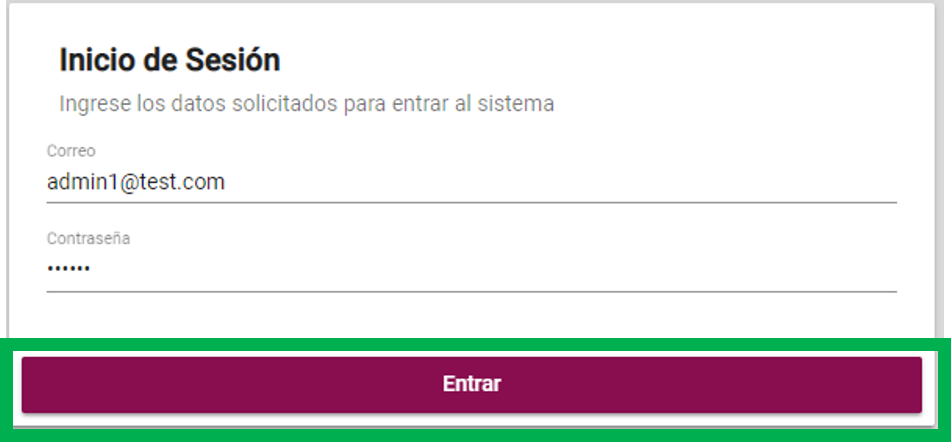
\includegraphics[width=0.5\linewidth]{images/SP5/BotonIngresar}}
            \caption{Botón de ingresar}
            %\label{consultarrh}
        \end{figure}

        Si el correo y la contraseña son correctos entonces podrá ver la página principal del sistema:

        % Imagen de Pagina principal
        \begin{figure}[!hbtp]
            \centering
            \hypertarget{Principal}{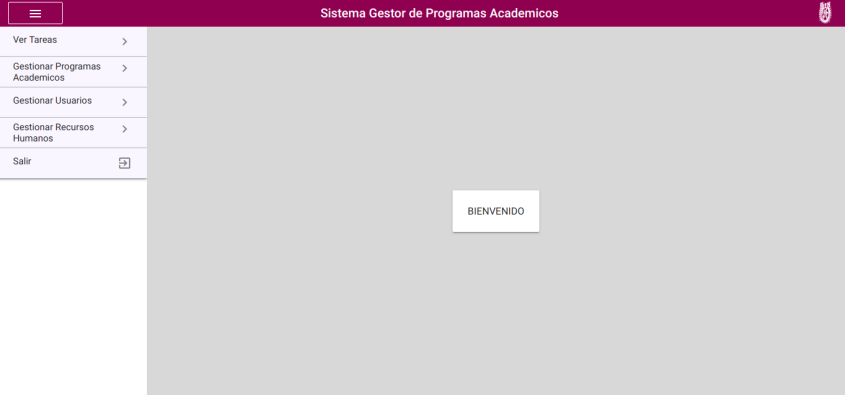
\includegraphics[width=0.7\linewidth]{images/SP5/Principal}}
            \caption{Pantalla principal}
            %\label{consultarrh}
        \end{figure}

        \clearpage
        \subsubsection{Posibles errores}

            \begin{itemize}
                \item La página no esta disponible.

                    Al suceder esto, aparecerá el siguiente mensaje:
                    % Imagen del mensaje  Por el momento no esta disponible
                    \begin{figure}[!hbtp]
                        \centering
                        \hypertarget{MSG25}{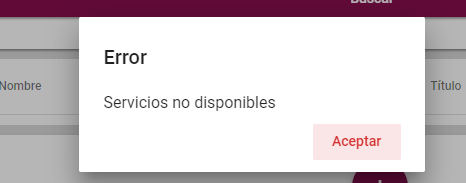
\includegraphics[width=0.4\linewidth]{images/SP5/MSGSN}}
                        \caption{Mensaje de servicios no disponibles}
                        %\label{consultarrh}
                    \end{figure}

                    Significa que existió un error de conexión o del sistema. Al dar clic en en botón ''Aceptar'', usted continuará en la pantalla de \hyperlink{iniciarL}{\textit{Iniciar Sesión}}. Deberá esperar a que la página este disponible para intentar acceder nuevamente.

                \item Correo y/o contraseña incorrectas, o se dejo algún campo vacío.
                    % Imagen del mensaje
                    \begin{figure}[!hbtp]
                        \centering
                        \hypertarget{MSG0}{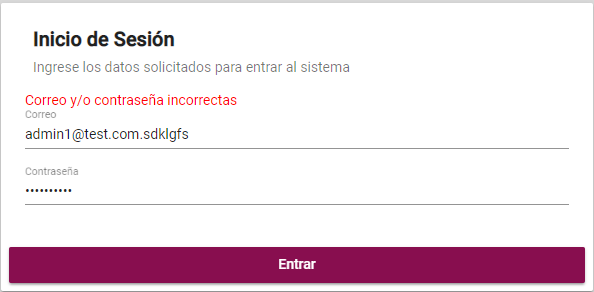
\includegraphics[width=0.4\linewidth]{images/SP5/LoginIncorrecto}}
                        \caption{Mensaje de datos incorrectos}
                        %\label{consultarrh}
                    \end{figure}

                Significa que la composición de los datos ingresados no es la correcta. Tenga en cuenta lo siguiente:

                            \begin{itemize}
                                \item Debe estar previamente registrado en el sistema.
                                \item El correo electrónico debe ser el otorgado por su jefe directo.
                                \item La contraseña no acepta acentos, espacios o caracteres especiales.
                                \item Ninguno de ambos campos debe dejarse vacío.
                            \end{itemize}

            \end{itemize}
